% this file is called up by thesis.tex
% content in this file will be fed into the main document

% change according to folder and file names
\ifpdf
    \graphicspath{{figures/}{figures/comparisons}}
\else
    \graphicspath{{figures/}{figures/comparisons}}
\fi


\chapter{Evaluation} % top level followed by section, subsection
All implemented algorithms were tested in terms speed, accuracy and effectiveness. For speed test normal processor execution time were measured. For accuracy Sampson Error was used(point distance to corresponding epipolar line in image). For effectivness visual comparison of reconstructed 3D cloud points was used.
% ----------------------- contents from here ------------------------
\section{Acquiering datasets}
Following datasets were captured with implemented "Sensor Enhanced Images Camera" and Nexsus 5 camera:
\begin{enumerate}
\item Warsaw University of technology main building(4 images 1024x768pixels)
\item Advertisment Pole ??? 
\item Warsaw Buisness School Gate and Entrance ??
\item Warsaw Shopping Center Back???
\item Warsaw Shopping Center Front???
\end{enumerate}
As most of proposed algorithms require that Intersic Camera Parametrs are known, also used camera was calibrated and its parameters stored in $"out_camera_data.yml"$ file. All of these datasets can be found on attached CD or Github repository.
\section{Test Environment}
All test were perfomed on MacBook Air with 1.7GHz dual-core Intel Core i7 processor and 8GB 1600MHz DDR3 RAM using implemented "Enhanced 3D Reconstructer".  Numerical tests, which allowed to measure Total Errors and execution time were run on "Waraw University of Technology" dataset. Also  reconstruction ability of each proposed methods was measured and different reconstruction strategies as well.  Finally for each dataset most promising Enhanced 8-point method was used to reconstruct sparse models. 
\section{Testing two-view reconstrucion methods} \label{sec:Testin2Views}
The most important thing to determine was to evaluate, wether proposed sensor enhanced improvements scored better than normal algorithms.
Following methods were tested: TODO methods should be already described in Concept and implementation
\begin{enumerate}
\item \textbf{Standard 8-point} - based on [] Fundamental matrix decomposition, implemented in OpenCV
\item \textbf{Enhanced 8-point} - proposed camera rotation enhanced version of above 8-point algorithm
\item \textbf{Alternative 3-point} - proposed 3-point algorithm to translation estimation.
\item \textbf{Known rotations and translations} - calculation from known cameras rotations and translations
\item \textbf{Standard essential 5-point} - based on [] Essential matrix decomposition, implemented in []
\item \textbf{Enhanced essential 5-point} - similar to 2. improvements rotation enhanced version of above 5-point algorithm
\end{enumerate}
\subsection{Accuracy - Epipolar lines correspondence}
In terms of two pair images one of the most imporant factors is the epipolar constraint. With properly estimated Fundamental matrix we can draw in both images corresponding epipolar lines. What's more points that lie on two matching epipolars line can be easily matched. Simply speaking epipolar line crosses exactly the same points in both images. The more accurate it it the more corresponding pairs can be later found for instance to perform dense reconstraction. Sampson Error[reference]is one of metrics, that can be used in order to estimate, how accurate epipolars line are. 
\begin{figure}[b!]
  \begin{center}
    \begin{tikzpicture}
      \begin{axis}[
          width=\linewidth, % Scale the plot to \linewidth
          grid=major, % Display a grid
          grid style={dashed,gray!30}, % Set the style
          xtick = {100,500,1000,5000},
          xlabel=Sift features number, % Set the labels
          xmode=log,
          log ticks with fixed point,
          ymode=log,
          log ticks with fixed point,
          ylabel=Total Sampson Error(pixels),
          legend style={at={(0.5,-0.05)},anchor=north,cells={anchor=west}}, % Put the legend below the plot
        ]
        \addplot[mark=*,blue] table[x=Number of Sift features,y=8-point OpenCV,col sep=comma] {SampsonTotal.csv}; 
        \addplot[mark=*,red] table[x=Number of Sift features,y=8-point enhanced,col sep=comma] {SampsonTotal.csv};
        \addplot[mark=*,orange] table[x=Number of Sift features,y=Alternative 3-point,col sep=comma] {SampsonTotal.csv}; 
        \addplot[mark=*,pink] table[x=Number of Sift features,y=Known rot and trans,col sep=comma] {SampsonTotal.csv};
        \addplot[mark=*,green] table[x=Number of Sift features,y=Essential 5-point,col sep=comma] {SampsonTotal.csv};
        \addplot[mark=*,yellow] table[x=Number of Sift features,y=5-point enhanced,col sep=comma] {SampsonTotal.csv};
        \legend{Standard 8-point,Enhanced 8-point,Alternative 3-point,Known rotations and translations,Standard essential 5-point,Enhanced essential 5-point}
      \end{axis}
    \end{tikzpicture}
    \caption{Plot of total Sampson Error in picture(1024x768pixels) in comparison to initial Sift feature number}
    \label{plot:TotalSampsonError}
  \end{center}
\end{figure}
It basicly measures sum of all points distances to theirs corresponding epipolar lines. However each of proposed methods has different outliers removal capabilities. That's why also Samson Error Per Corresponding Pair was used.
On plot \ref{plot:TotalSampsonError} were visualized calculated total sampson errors for different initial SIFT features sets. Knowing that Total Sampson Error were calculated for different number of final inliers the only thing that can be noted here that most of the algoritms properly filter out outliers. Obviously drawing epipolar lines from heuristicaly estimated movement and noisy rotation gives extremly large error in comparison to others.
\begin{figure}[hb!]
  \begin{center}
    \begin{tikzpicture}
      \begin{axis}[
          width=\linewidth, % Scale the plot to \linewidth
          grid=major, % Display a grid
          grid style={dashed,gray!30}, % Set the style
          xtick = {100,500,1000,5000},
          xlabel=Sift features number, % Set the labels
          xmode=log,
          log ticks with fixed point,
          ymode=log,
          log ticks with fixed point,
          ylabel=Total Sampson Error per point(pixels),
          legend style={at={(0.5,-0.05)},anchor=north,cells={anchor=west}}, % Put the legend below the plot
        ]
        \addplot[mark=*,blue] table[x=Number of Sift features,y=8-point OpenCV,col sep=comma] {SampsonPerPoint.csv}; 
        \addplot[mark=*,red] table[x=Number of Sift features,y=8-point enhanced,col sep=comma] {SampsonPerPoint.csv};
        \addplot[mark=*,orange] table[x=Number of Sift features,y=Alternative 3-point,col sep=comma] {SampsonPerPoint.csv}; 
        \addplot[mark=*,pink] table[x=Number of Sift features,y=Known rot and trans,col sep=comma] {SampsonPerPoint.csv};
        \addplot[mark=*,green] table[x=Number of Sift features,y=Essential 5-point,col sep=comma] {SampsonPerPoint.csv};
        \addplot[mark=*,yellow] table[x=Number of Sift features,y=5-point enhanced,col sep=comma] {SampsonPerPoint.csv};
        \legend{Standard 8-point,Enhanced 8-point,Alternative 3-point,Known rotations and translations,Standard essential 5-point,Enhanced essential 5-point}
      \end{axis}
    \end{tikzpicture}
    \caption{Plot of per point Sampson Error in picture(1024x768pixels) in comparison to initial Sift feature number}
    \label{plot:SampsonErrorPerPoint}
  \end{center}
\end{figure}
Taking a look at Per Pair Sampson Error \ref{plot:SampsonErrorPerPoint} one can note that proposed sensor enhanced versions neither had improved 8-point nor 5-point algorithm. However proposed 3-point algorithm, which was much faster than 8-point algorithm turned out to be quite accurate. To present the reader, of what errors are we talking about on figures \ref{fig:SummaryEpiLines1300} - \ref{fig:SummaryEpiLines2300} estimated epipolar lines for 300 initial SIFT features were drawn. 
\begin{figure}[b!]
    \centering
    \includegraphics[width=0.8\textwidth]{summary1Sift300}
    \caption{Results of drawing estimated Epipolar lines on Warsaw Univeristy Dataset for 300 Sift points. 1) Standard Fundamental 8-point(upper pair), 2) Rotation Enhanced Fundamental 8-point(middle), 3) Alternative 3-point algorithm(bottom) }
    \label{fig:SummaryEpiLines1300}
\end{figure}
\begin{figure}[ht!]
    \centering
    \includegraphics[width=0.8\textwidth]{summary2Sift300}
    \caption{Results of drawing estimated Epipolar lines on Warsaw Univeristy Dataset for 300 Sift points. 1) Fundamental matrix created from rotation and translation(upper pair), 2) Standard Essential matrix 5-point(middle), 3)Rotation Enhanced Essential 5-point(bottom) }
    \label{fig:SummaryEpiLines2300}
\end{figure}
It can be seen that both Standard 8-point algorithm and proposed Rotation Enhanced version give very good results in term of epipolar lines. Alternative 3-point algorithm gives slightly worse results having good direction of lines, but due to uncompansated mobile sensors noise slightly incorrect. In these particular dataset Essential 5-point method in really sparse datasets had some problems in Essential matrix estimation, but our proposed imporved 5-point version found pretty good corresponding sets. To check if number of SIFT features influence these visualization epipolar calculation was also presented on 1000 SIFT features(\ref{fig:SummaryEpiLines11000} - \ref{fig:SummaryEpiLines21000}). 
\begin{figure}[b!]
    \centering
    \includegraphics[width=0.8\textwidth]{summary1Sift1000}
    \caption{Results of drawing estimated Epipolar lines on Warsaw Univeristy Dataset for 1000 Sift points. 1) Standard Fundamental 8-point(upper pair), 2) Rotation Enhanced Fundamental 8-point(middle), 3) Alternative 3-point algorithm(bottom) }
    \label{fig:SummaryEpiLines11000}
\end{figure}
\begin{figure}[ht!]
    \centering
    \includegraphics[width=0.8\textwidth]{summary2Sift1000}
    \caption{Results of drawing estimated Epipolar lines on Warsaw Univeristy Dataset for 1000 Sift points. 1) Fundamental matrix created from rotation and translation(upper pair), 2) Standard Essential matrix 5-point(middle), 3)Rotation Enhanced Essential 5-point(bottom) }
    \label{fig:SummaryEpiLines21000}
\end{figure}
Generally proposed improvements versions aren't better in terms of accuracy due to noise in data sensors, however they are always close to optimal solutions, when standard versions can fail sometimes.
\clearpage

\subsection{Time comparison}
As was mentioned in previos chapter we expect some of this methods to be faster than the others. On plot \ref{plot:ExecutionTime} avaraged  execution time for 100 attempts was presented. 
\begin{figure}[hb!]
  \begin{center}
    \begin{tikzpicture}
      \begin{axis}[
          width=\linewidth, % Scale the plot to \linewidth
          grid=major, % Display a grid
          grid style={dashed,gray!30}, % Set the style
          xtick = {100,500,1000,5000},
          xlabel=Sift features number, % Set the labels
          xmode=log,
          log ticks with fixed point,
          ymode=log,
          ylabel=Execution time(ms),
          legend style={at={(0.5,-0.05)},anchor=north,cells={anchor=west}}, % Put the legend below the plot
        ]
        \addplot[mark=*,blue] table[x=Number of Sift features,y=8-point OpenCV,col sep=comma] {ExecutionTime.csv}; 
        \addplot[mark=*,red] table[x=Number of Sift features,y=8-point enhanced,col sep=comma] {ExecutionTime.csv};
        \addplot[mark=*,orange] table[x=Number of Sift features,y=Alternative 3-point,col sep=comma] {ExecutionTime.csv}; 
        \addplot[mark=*,pink] table[x=Number of Sift features,y=Known rot and trans,col sep=comma] {ExecutionTime.csv};
        \addplot[mark=*,green] table[x=Number of Sift features,y=Essential 5-point,col sep=comma] {ExecutionTime.csv};
        \addplot[mark=*,yellow] table[x=Number of Sift features,y=5-point enhanced,col sep=comma] {ExecutionTime.csv};
        \legend{Standard 8-point,Enhanced 8-point,Alternative 3-point,Known rotations and translations,Standard essential 5-point,Enhanced essential 5-point}
      \end{axis}
    \end{tikzpicture}
    \caption{Execution time of proposed algorithms(1024x768pixels) in comparison to initial Sift feature number}
    \label{plot:ExecutionTime}
  \end{center}
\end{figure}
As expected reconstructing using known rotations and translations is few orders smaller than rest algorithms. Also 3-point algorithm execution time is few times smaller than 8-point algorithms. Execution time of 8-point versions are very similar, but 5-point versions differ much. Either finding optimal solution with initial rotation is much harder or implementation differences in memory allocation of enhanced versions takes a lot of additional time.

\section{Testing reconstruction strategies}
As was seen in \ref{sec:Testin2Views} not every initial reconstruction gives good results. To keep clearness of this document only most promising and interesting strategies were used: TODO methods should be already described in Concept and implementation
\begin{enumerate}
\item \textnormal{Standard 8-point + OpenCV Pose Estimation} 
\item \textnormal{Enhanced 8-point + OpenCV Pose Estimation} 
\item \textnormal{Enhanced 8-point + Initial Rotation and Translation OpenCV Pose Estimation} 
\item \textnormal{Alternative 3-point + OpenCV Pose Estimation}
\item \textnormal{Alternative 3-point + Initial Rotation and Translation OpenCV Pose Estimation}
%\item \textnormal{Known rotations and translations} 
\end{enumerate}
First method gives us basic reference to normal 3D reconstruction pipeline. 2nd and 3rd were used in order to check how Pose Estimation enhancment influence final results. 4th and 5th one were compared with 2nd-3rd strategies. Finally 6th one was proposed in order to check, how well reconstraction can be performed with only sensor data.

\subsection{Accuracy}
Accuracy of 3D reconstraction were measured using Bundle Adjustment process from SBA library[ref]. At the beginning initial error of whole point cloud is calculated. What's more to better understand, how well models were reconstructed it's intresting to take a look at both model error reduction and BA execution time.
For "Warsaw Univeristy" dataset performed performence tests were plotted on \ref{plot:BAError}. Big differences in Initial Error mainly lay in number of reconstructed points and scale of models, which turned out to be more very different due to differences in outlier removals. What's interesting is impact of enhancing reconstruction with initial rotations and translation on Bundle Adjustments. 
\begin{figure}[ht!]
  \begin{center}
    \begin{tikzpicture}
      \begin{axis}[
          width=\linewidth, % Scale the plot to \linewidth
          grid=major, % Display a grid
          grid style={dashed,gray!30}, % Set the style
          xtick = {1,2,3,4,5},
          xticklabels = {Std8 -point+NormalPose,Enhanced8-point+NormalPose,Enhanced8-point+EnhancedPose, Alternative3-point+NormalPose,Alternative3-point+EnhancedPose},          
          xlabel=Reconstruction strategy, % Set the labels
          log ticks with fixed point,
          ymode=log,
          ylabel=Reconstruction error(in model units),
          x tick label style={rotate=90,anchor=east},
          legend style={at={(0.5,1.05)},anchor=south,cells={anchor=west}}, % Put the legend below the plot
        ]
        \addplot[mark=*,blue] table[x=ReconMethods,y=Error before BA,col sep=comma] {BAerror2.csv}; 
        \addplot[mark=*,red] table[x=ReconMethods,y=Error after BA,col sep=comma] {BAerror2.csv};
        \legend{Reconstruction Error before Bundle Adjustment,Reconstruction Error after Bundle Adjustment}
      \end{axis}
    \end{tikzpicture}
    \caption{Comparison of different reconstruction strategies influence on Bundle Adjustment}
    \label{plot:BAError}
  \end{center}
\end{figure}
\clearpage
Bundle Adjustmet process allows to rearrange both estimated 3D points positions and positions of the cameras. When camera positions are close to their true,optimal positions it allows algorithms to focus on 3D points movement refinments. What's more Rotation and Translation enhanced position estimation has further influence in reduction of final BA error in comparison to Normal Pose Estimation. 


%\begin{figure}[h]
%  \begin{center}
%    \begin{tikzpicture}
%      \begin{axis}[
%          width=\linewidth, % Scale the plot to \linewidth
%          grid=major, % Display a grid
%          grid style={dashed,gray!30}, % Set the style
%          xtick = {100,500,1000,5000},
%          xlabel=Sift features number, % Set the labels
%          xmode=log,
%          log ticks with fixed point,
%          ymode=normal,
%          ylabel=Execution time(ms),
%          legend style={at={(0.5,-0.2)},anchor=north,cells={anchor=west}}, % Put the legend below the plot
%        ]
%        \addplot[mark=*,blue] table[x=Number of Sift features,y=8-pointInit+NormalPoseEstim,col sep=comma] {ReconstructInit.csv}; 
%        \addplot[mark=*,red] table[x=Number of Sift features,y=Enhanced8-point+NormalPoseEstim,col sep=comma] {ReconstructInit.csv};
%        \addplot[mark=*,orange] table[x=Number of Sift features,y=Enhanced8-point+EnhancedPoseEstim,col sep=comma] {ReconstructInit.csv}; 
%        \addplot[mark=*,pink] table[x=Number of Sift features,y=Alternative3-point+NormalPoseEstim,col sep=comma] {ReconstructInit.csv};
%        \addplot[mark=*,green] table[x=Number of Sift features,y=Alternative3-point+EnhancedPoseEstim,col sep=comma] {ReconstructInit.csv};
%        \addplot[mark=*,yellow] table[x=Number of Sift features,y=Known Rotations and Translations,col sep=comma] {ReconstructInit.csv};
%        \legend{Standard 8-point initialization + Normal OpenCV Pose Estimation,Enhanced 8-point initialization + Normal Pose Estimation,Enhanced 8-point initiazliation + Enhanced Pose Estim, Alternative 3-point initiazliation + Normal Pose Estimation, Alternative 3-point initialization + Enhanced Pose Estimation, Known Rotations and Translations}
%      \end{axis}
%    \end{tikzpicture}
%    \caption{Execution time of first pair images recontruction(1024x768pixels) in comparison to initial Sift feature number}
%  \end{center}
%\end{figure}
\subsection{Execution time}
To see how proposed algorithms improve reconstruction process execution time without Bundle Adjustment was measured in \ref{plot:ReconstructionWithoutBA}. What can be noted that in comparison to Epipolar lines estimation overall reconstruction process time was slightly improved especially with 3-point algorithms. Comparing it to Execution times in \ref{plot:ExecutionTime} one can see that most of this time is used for SIFT correspondences matching, which is bottle-neck in proposed reconstruction methodology[reference to concept pose esitmation choosing]. Also Reconstruction time was also measered with Bundle Adjustment process at the end(\ref{plot:ReconstructionWithBA}). It turns out that Bundle Adjustment works much better on with enhanced Initial Pait reconstruction and Pose Estimation. Such cloud points are much better organised than standard reconstructed ones, which results in faster convergence of BA. Sample difference between cloud points before and after BA can be seen in \ref{fig:BundleAdjustmentComparison}
\begin{figure}[b!]
    \centering
    \includegraphics[width=\textwidth]{bundleAdjustmentComparison}
    \caption{3D point clouds before Bundle Adjustment(upper) and after(bottom) for Enhanced 8-point with Enhanced Pose Estimation. Warsaw University of Technology dataset for 1000 SIFT corresponding features(left - front, right - from side)}
    \label{fig:BundleAdjustmentComparison}
\end{figure}
\begin{figure}[h!]
  \begin{center}
    \begin{tikzpicture}
      \begin{axis}[
          width=\linewidth, % Scale the plot to \linewidth
          grid=major, % Display a grid
          grid style={dashed,gray!30}, % Set the style
          xtick = {100,500,1000,5000},
          xlabel=Sift features number, % Set the labels
          xmode=log,
          log ticks with fixed point,
          ymode=normal,
          ylabel=Execution time(ms),
          legend style={at={(0.5,-0.05)},anchor=north,cells={anchor=west}}, % Put the legend below the plot
        ]
        \addplot[mark=*,blue] table[x=Number of Sift features,y=8-pointInit+NormalPoseEstim,col sep=comma] {ReconstructTotal.csv}; 
        \addplot[mark=*,red] table[x=Number of Sift features,y=Enhanced8-point+NormalPoseEstim,col sep=comma] {ReconstructTotal.csv};
        \addplot[mark=*,orange] table[x=Number of Sift features,y=Enhanced8-point+EnhancedPoseEstim,col sep=comma] {ReconstructTotal.csv}; 
        \addplot[mark=*,pink] table[x=Number of Sift features,y=Alternative3-point+NormalPoseEstim,col sep=comma] {ReconstructTotal.csv};
        \addplot[mark=*,green] table[x=Number of Sift features,y=Alternative3-point+EnhancedPoseEstim,col sep=comma] {ReconstructTotal.csv};
%        \addplot[mark=*,yellow] table[x=Number of Sift features,y=Known Rotations and Translations,col sep=comma] {ReconstructTotal.csv};
        \legend{Standard 8-point initialization + Normal OpenCV Pose Estimation,Enhanced 8-point initialization + Normal Pose Estimation,Enhanced 8-point initiazliation + Enhanced Pose Estim, Alternative 3-point initiazliation + Normal Pose Estimation, Alternative 3-point initialization + Enhanced Pose Estimation}
      \end{axis}
    \end{tikzpicture}
    \caption{Total reconstruction execution time (4 images with resolution 1024x768pixels) in comparison to Sift feature number}
    \label{plot:ReconstructionWithoutBA}
  \end{center}
\end{figure}

%TODO Interesting thing that pose estimation time is relativly small to correspondence matching. The same with triangulation it\'s quick.\newline
\begin{figure}[h!]
  \begin{center}
    \begin{tikzpicture}
      \begin{axis}[
          width=\linewidth, % Scale the plot to \linewidth
          grid=major, % Display a grid
          grid style={dashed,gray!30}, % Set the style
          xtick = {100,500,1000,5000},
          xlabel=Sift features number, % Set the labels
          xmode=log,
          log ticks with fixed point,
          ymode=normal,
          ylabel=Execution time(ms),
          scaled ticks = false,
          xticklabel style={/pgf/number format/.cd,fixed,precision=5},
          legend style={at={(0.5,-0.05)},anchor=north,cells={anchor=west}}, % Put the legend below the plot
        ]
        \addplot[mark=*,blue] table[x=Number of Sift features,y=8-pointInit+NormalPoseEstim,col sep=comma] {ReconstructBA.csv}; 
        \addplot[mark=*,red] table[x=Number of Sift features,y=Enhanced8-point+NormalPoseEstim,col sep=comma] {ReconstructBA.csv};
        \addplot[mark=*,orange] table[x=Number of Sift features,y=Enhanced8-point+EnhancedPoseEstim,col sep=comma] {ReconstructBA.csv}; 
        \addplot[mark=*,pink] table[x=Number of Sift features,y=Alternative3-point+NormalPoseEstim,col sep=comma] {ReconstructBA.csv};
        \addplot[mark=*,green] table[x=Number of Sift features,y=Alternative3-point+EnhancedPoseEstim,col sep=comma] {ReconstructBA.csv};
%        \addplot[mark=*,yellow] table[x=Number of Sift features,y=Known Rotations and Translations,col sep=comma] {ReconstructTotal.csv};
        \legend{Standard 8-point initialization + Normal OpenCV Pose Estimation,Enhanced 8-point initialization + Normal Pose Estimation,Enhanced 8-point initiazliation + Enhanced Pose Estim, Alternative 3-point initiazliation + Normal Pose Estimation, Alternative 3-point initialization + Enhanced Pose Estimation}
      \end{axis}
    \end{tikzpicture}
    \caption{Total execution time of reconstruction with Bundle Adjustment(4 images with resolution 1024x768pixels) in comparison to Sift feature number}
    \label{plot:ReconstructionWithBA}
  \end{center}
\end{figure}
\clearpage

\section{Effectivness}
However numerical measuerments do not always results in proper 3D model reconstructions, so some of the intresting 3D reconstraction situations are presented on next 4 pages. In \ref{fig:uni4000Comparison} different Initialization Pair methods were used to reconstruction models for 4000 SIFT features. It can be seen that standard and enhaced methods gave quite good results, which only differ in scale. 3-point algorithm produces quite good models, but slightly distorted due to noise in used rotations. Model reconstructed from known rotations and translations are very distorted, but stil readable. It could be used, when very fast reconstruction is needed. Essential Matrix estimation methods unfortunately failed in terms of relative pose estimation.
\newline
However situation changes a little bit for 400 points. Every algorithm managed to find solution reallt close to optimum. In some cases "Traingulation Test" used in Standard 8-point approach fails and produces unrecognizable model(\ref{fig:FailCaseFundamental}).
\newline
When it comes to Pose Estimations enhancments one can see in \ref{fig:PoseEstimationMethodComparison} that generally initial  rotation and translation help to find better solution, which mainly manifests in less outliers number.
\newline
In figure \ref{fig:UniNone4000} it can be seen, how many outliers using only noisy rotations and translations produces.
\newline
More reconstructed models can be found in [TODO Materials]
\begin{figure}[p]
    \centering
    \includegraphics[width=0.9\textwidth]{uni4000Comparison}
    \caption{Reconstructed models for proposed Initial reconstruction methods and 4000 Sift Features. From upper left to bottom right following: 1) Standard 8-point, 2) Enhanced 8-point, 3) Alternative 3-point, 4) Known rotations and translations, 5) Standard 5-point, 6) Enhanced 5-point}
    \label{fig:uni4000Comparison}
\end{figure}
\begin{figure}[t!]
    \centering
    \includegraphics[width=0.9\textwidth]{uni400Comparison}
    \caption{Reconstructed models for proposed Initial reconstruction methods and 400 Sift Features. From upper left to bottom right following: 1) Standard 8-point, 2) Enhanced 8-point, 3) Alternative 3-point, 4) Known rotations and translations, 5) Standard 5-point, 6) Enhanced 5-point}
    \label{fig:uni400Comparison}
\end{figure}
\begin{figure}[p]
    \centering
    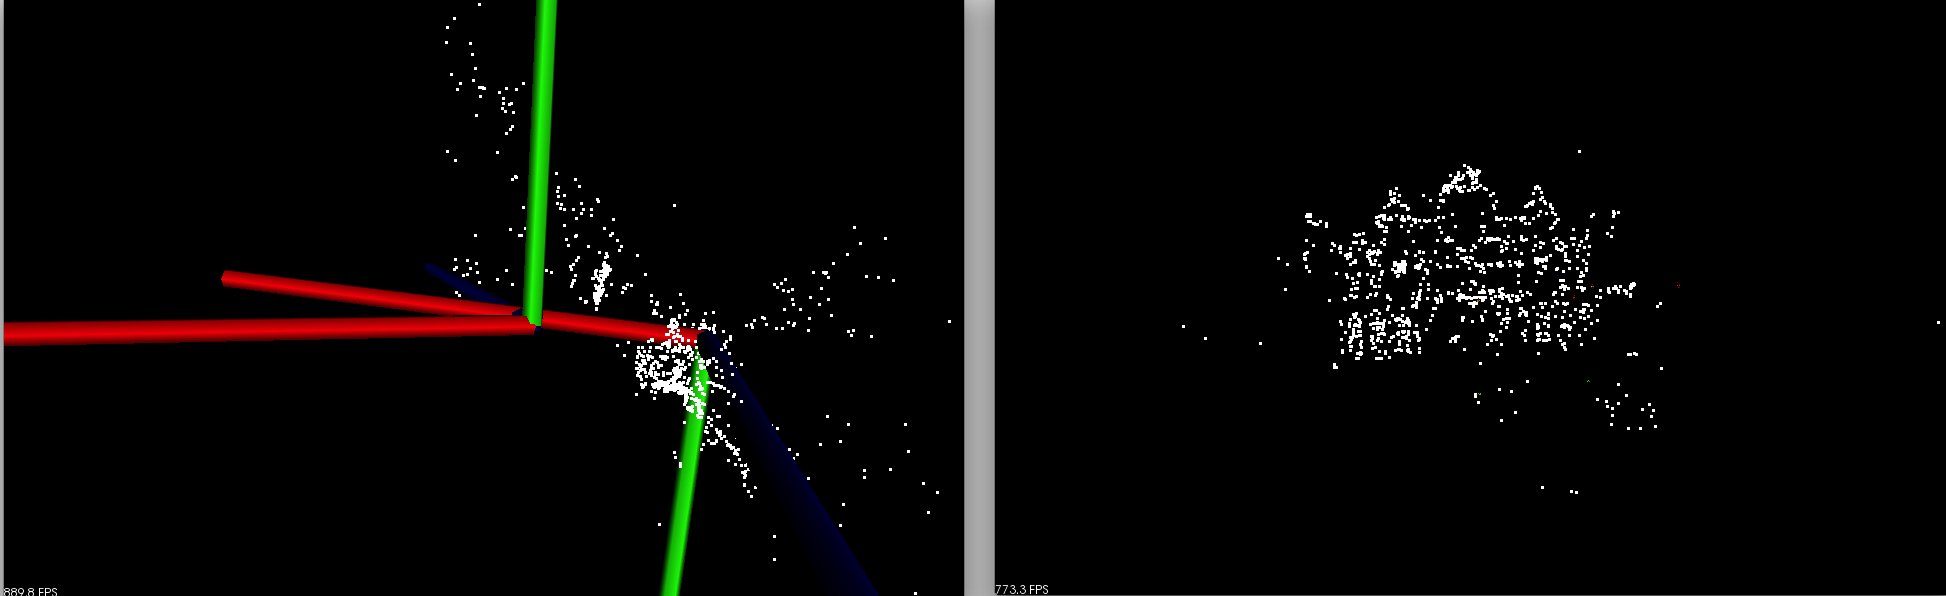
\includegraphics[width=0.9\textwidth]{FailCaseFundamental}
    \caption{Fail test case of Standard 8-point triangulation(left) in comparison to fortunate reconstruction}
    \label{fig:FailCaseFundamental}
\end{figure}
\begin{figure}[p]
    \centering
    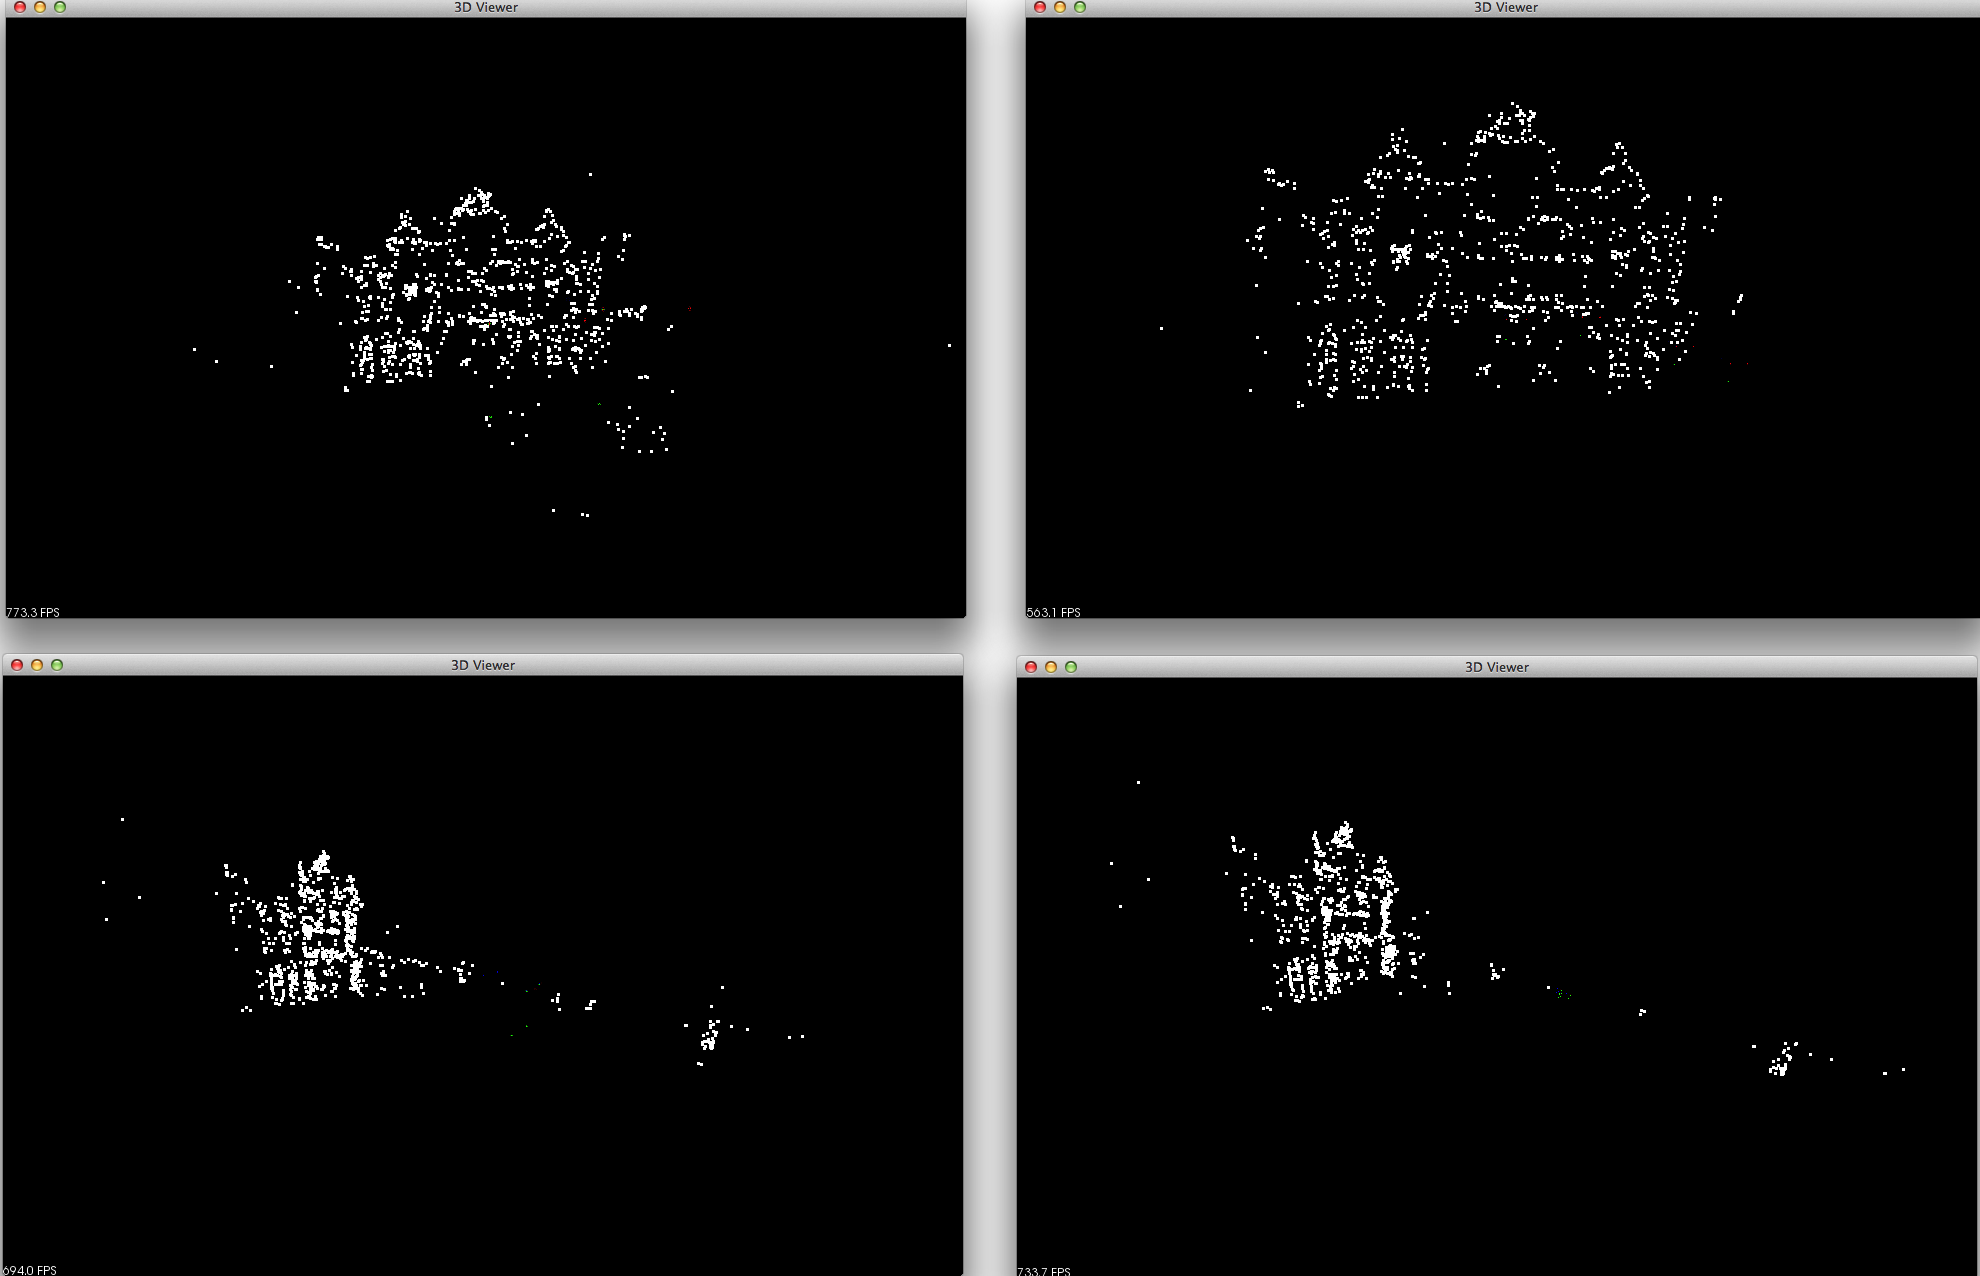
\includegraphics[width=0.9\textwidth]{PoseEstimationMethodComparison}
    \caption{Pose estimation methods comparison(Views from front and side). Left: Normal Pose Estimation, right: Enhanced Rotation and Translation Pose Estimation}. Less outliers are reconstructed when enhancment is used.
    \label{fig:PoseEstimationMethodComparison}
\end{figure}
\begin{figure}[p]
    \centering
    \includegraphics[height=18cm]{uniNone4000}
    \caption{Reconstruction results from known translations and rotations from different angles. Upper shows front face of building, other from different angles. Many outliers in reconstructed model.}
    \label{fig:UniNone4000}
\end{figure}

% ---------------------------------------------------------------------------
% ----------------------- end of thesis sub-document ------------------------
% ---------------------------------------------------------------------------